\documentclass[a4paper, 12pt]{article}
\usepackage[top=2.5cm,
            left=3.5cm,
            right=1.5cm,
            bottom=2.5cm,
            includefoot]{geometry}              % set margins

% LANGUAGE %
%-========-%
\usepackage{luavlna}                            % auto non-breaking spaces
\AtBeginDocument{\singlechars{czech}{AaIiVvOoUuSsZzKk}}
\usepackage[czech]{babel}                       % use the czech language


% TOC AND LOF %
%-===========-%
\usepackage[subfigure, titles]{tocloft}         % controlling lof and lot
\usepackage[nottoc]{tocbibind}                  % no toc in toc

\makeatletter                                   % remove titles from lof and lot
\renewcommand\listoffigures{%
    \@mkboth{\MakeUppercase\listfigurename}%
        {\MakeUppercase\listfigurename}%
    \@starttoc{lof}%
}
\renewcommand\listoftables{%
    \@mkboth{\MakeUppercase\listtablename}%
        {\MakeUppercase\listtablename}%
    \@starttoc{lot}%
}
\makeatother

\setlength{\cftfigindent}{0pt}                  % no lof indentation
\setlength{\cfttabindent}{0pt}                  % no lot indentation

\renewcommand{\contentsname}{Obsah}             % change toc name

\usepackage{setspace}                           % for making a more concise toc


% CODE %
%-====-%
\usepackage{minted}


% GRAPHICS %
%-========-%
\usepackage{graphicx}                           % graphics package
\graphicspath{ {./img/} }                       % graphics path

\usepackage{float}                              % floats in correct position
\usepackage{subfig}                             % subfigure package

\setlength{\fboxsep}{0pt}                       % image border separation
\setlength{\fboxrule}{0.5pt}                    % image border thickness


% CROSS-REFERENCES %
%-================-%
\usepackage[hyphens,spaces,obeyspaces]{url}     % url
\usepackage[hidelinks,unicode]{hyperref}        % interactive links
\newcommand*{\fullref}[1]{\hyperref[{#1}]{\ref*{#1}}}


% BIBLIOGRAPHY %
%-============-%
\usepackage[backend=biber,
            style=iso-numeric,
            sortlocale=cs_CZ,
            autolang=other,
            bibencoding=UTF8]{biblatex}         % use BibLaTeX for references
\addbibresource{soc.bib}                        % reference file

\renewcommand*{\finentrypunct}{}                % don't end the reference with .
\renewcommand{\multinamedelim}{\addcomma\space} % use comma as delimeter
\renewcommand{\finalnamedelim}{\addspace a \space} % use a as final name delim
\renewbibmacro{in:}{}                           % don't use In:

\DeclareFieldFormat{labelnumberwidth}{[#1]}     % wrap refs in square brackets


% TABLES          %
% requires: float %
%-===============-%
\floatstyle{plaintop}                           % table caption on top
\restylefloat{table}                            % -||-
\usepackage{booktabs}                           % table formatting


% MISCELLANEOUS %
%-=============-%
\usepackage{amsmath, amstext}                   % math

\usepackage[font=small,
            labelfont=bf,
            figurename=Obr.,
            tablename=Tab.,
            belowskip=-12pt]{caption}           % captions

\usepackage{enumitem}                           % lists


% DATETIME %
%-========-%
\usepackage[dmyyyy]{datetime}                   % dmyyyy datetimes
\renewcommand{\dateseparator}{. }               % changes datetime separator


% FONT AND ENCODING %
%-=================-%
\usepackage[T1]{fontenc}                        % font encoding
\usepackage{fontspec}                           % font selector

\setmainfont{CMU Serif}                         % a font that suports bx sc


% ACRONYMS %
%-========-%
\usepackage[acronym,                            % use acronyms
            nopostdot,                          % no dot at end of 2nd column
            numberedsection,                    % number glossary
            nogroupskip,                        % no grouping by same letter
            nonumberlist]{glossaries}           % no page numbers

\renewcommand{\acrfullformat}[2]{#2\space(#1)}  % long (short) to short (long)

\setglossarystyle{alttree}                      % set style of glossary

% make glossary title spacing be the same as regular title
\renewcommand{\glossarypreamble}{\vspace*{-\baselineskip}\vspace*{-\parskip}}

\makeglossaries

\newacronym{frc}{FRC}{First Robotics Competition}
\newacronym{ftc}{FTC}{First Technical Challenge}
\newacronym{fll}{FLL}{First Lego League}
\newacronym{pdf}{PDF}{Portable Document Format}
\newacronym{html}{HTML}{Hypertext Mark-up Language}
\newacronym{cern}{CERN}{Evropská organizace pro jaderný výzkum}
\newacronym{http}{HTTP}{Hypertext Transfer Protocol}
\newacronym{css}{CSS}{Cascading Style Sheets}
\newacronym{sass}{SASS}{Syntactically Awesome Style Sheets}
\newacronym{cvs}{CVS}{Concurrent Versions System}
\newacronym{cad}{CAD}{Computer-Aided Design}
\newacronym{ftp}{FTP}{File Transfer Protocol}
\newacronym{aes}{AES}{Advanced Encryption Standard}
\newacronym{api}{API}{Application Programming Interface}
\newacronym{si}{SI}{Mezinárodní systém jednotek}
\newacronym{ip}{IP}{Internet Protocol}
\newacronym{png}{PNG}{Portable Network Graphics}
\newacronym{wysiwyg}{WYSIWYG}{What You See Is What You Get}
\newacronym{php}{PHP}{Hypertext Preprocessor}
\newacronym{epub}{EPUB}{Electronic Publication}
\newacronym{mobi}{MOBI}{Mobipocket e-book}
\newacronym{mit}{MIT}{Massachusetts Institute of Technology}
\newacronym{it}{IT}{Information Technology}
\newacronym{www}{WWW}{World Wide Web}
\newacronym{sgml}{SGML}{Standard Generalized Mark-up Language}
\newacronym{https}{HTTPS}{Hypertext Transfer Protocol Secure}

\glsaddall                                      % add all acronyms
\glssetwidest{WYSIWYGGG}                        % manually set the widest acr.


% TEXT FORMATTING %
%-================-%
\usepackage{titlesec}

% titles have sizes 18pt, 16pt and 14pt, respectively
% the space between the number and the text of the title is 1em
\titleformat{\section}{\bfseries\scshape\fontsize{18pt}{21.6}\selectfont}{\thesection}{1em}{}
\titleformat{\subsection}{\bfseries\fontsize{16pt}{19.2}\selectfont}{\thesubsection}{1em}{}
\titleformat{\subsubsection}{\bfseries\fontsize{14pt}{16.8}\selectfont}{\thesubsubsection}{1em}{}

\setlength\parindent{0pt}                       % 0pt paragraph indentation
\setlength\parskip{12pt}                        % 12pt paragraph spacing

\titlespacing{\section}      {0pt}{0pt}{6pt}    % 18pt (12pt + 6pt)
\titlespacing{\subsection}   {0pt}{0pt}{4pt}    % 16pt (12pt + 4pt)
\titlespacing{\subsubsection}{0pt}{0pt}{2pt}    % 14pt (12pt + 2pt)

\renewcommand{\baselinestretch}{1.15}           % baseline stretch


% OTHER %
%-=====-%
\widowpenalty10000                              % prevent widows
\clubpenalty10000                               % prevent widows

\pagenumbering{gobble}                          % suppress page numbering

% define KaTeX logo
\makeatletter
\DeclareRobustCommand{\KaTeX}{%
  K\kern -.19em
  {\sbox \z@ T\vbox to\ht \z@ {\hbox{%
  \check@mathfonts
  \fontsize\sf@size\z@
  \selectfont A}%
  \vss}%
}\kern -.15em
\TeX}
\makeatother


\begin{document}
  % fixes some lines going to the margins
  \sloppy

  % first page's geometry is different
  \newgeometry{top=2.5cm, left=2.5cm, right=2.5cm, bottom=2.5cm}

  \bfseries

  \begin{center}
    {\fontsize{18}{21.6} \selectfont STŘEDOŠKOLSKÁ ODBORNÁ ČINNOST}\\%
    \vspace*{\baselineskip}
    {\fontsize{14}{16.8} \selectfont Obor č. 18: Informatika}\\%

    \topskip0pt
    \vspace{16em}
    {\fontsize{20}{24} \selectfont Robotika Jednoduše}%
    \vspace*{\fill}
  \end{center}

  \fontsize{16}{19.2} \selectfont
  Tomáš Sláma\\
  Liberecký Kraj
  \hfill
  Turnov 2019

  % the geometry for the rest of the document
  \newgeometry{top=2.5cm, left=3.5cm, right=1.5cm, bottom=2.5cm}

  \newpage
  \begin{center}
    {\fontsize{18}{21.6} \selectfont STŘEDOŠKOLSKÁ ODBORNÁ ČINNOST}\\%
    \vspace*{\baselineskip}
    {\fontsize{14}{16.8} \selectfont Obor č. 18: Informatika}\\%

    \topskip0pt
    \vspace{10em}
    \fontsize{20}{24} \selectfont
    Robotika Jednoduše%

    Robotics Simplified%
    \vspace*{\fill}
  \end{center}

  \normalfont
  \fontsize{16}{19.6} \selectfont

  \textbf{Autoři:} Tomáš Sláma\\
  \textbf{Škola:} Gymnázium, Turnov, Jana Palacha 804, příspěvková \\ organizace, 511 21 Turnov \\
  \textbf{Kraj:} Liberecký kraj \\
  \textbf{Konzultant:} Mgr. Tomáš Novotný

  \vspace{\baselineskip}

  \fontsize{12}{14.4} \selectfont
  Turnov 2019

  \vspace{4em}

  \newpage

  \section*{\normalfont\textbf{Prohlášení}}
  Prohlašuji, že jsem svou práci SOČ vypracoval/a samostatně a použil/a jsem pouze prameny a literaturu uvedené v seznamu bibliografických záznamů.

  Prohlašuji, že tištěná verze a elektronická verze soutěžní práce SOČ jsou shodné.

  Nemám závažný důvod proti zpřístupňování této práce v souladu se zákonem č.~121/2000 Sb., o právu autorském, o právech souvisejících s právem autorským a o změně některých zákonů (autorský zákon) ve znění pozdějších předpisů.

  \qquad

  V Turnově dne \today \, .......................................................\\%
  \makebox[\linewidth]{Tomáš Sláma}%

  \newpage

  \section*{\normalfont\textbf{Poděkování}}
  V první řadě bych rád poděkoval své rodině a přátelům za neustálou podporu a pozitivitu při tvorbě projektu. Za konzultace o obsahu, struktuře a v projektu použitých technologiích děkuji Mgr. Lukáši Pitoňákovi a Mgr. Tomáši Novotnému. Také děkuji Kateřině Sulkové za rady ke psaní samotné SOČ práce a na závěr všem návštěvníkům projektu, kteří svou přítomností a zpětnou vazbou pomáhají v jeho rozvoji.

  \newpage

  \section*{\normalfont\textbf{Anotace}}
  Tato práce popisuje proces tvorby webové stránky \url{robotics-simplified.com}. Stránka zpracovává témata z oboru robotiky formou pochopitelnou i naprostým začátečníkem. Je poháněna generátorem statických stránek Jekyll, který doplňují JavaSriptové knihovny pro vykreslování matematických rovnic, analýzy návštěvnosti a interaktivní vizualizaci probíraných konceptů. Python skripty automatizují kompresi obrázků, generování souboru sitemap, nahrání obsahu na hosting přes \acrshort{ftp} a převod stránky do knižní podoby pro offline čtení.

  \section*{\normalfont\textbf{Klíčová slova}}
  robotika; webová stránka; vzdělávání

  \section*{\normalfont\textbf{Annotation}}
  This paper decribes the process of creating the \url{robotics-simplified.com} website. The site covers topics in the field of robotics in a beginner-friendly way. It is powered by the static site generator Jekyll, and is suplemented by JavaScript libraries for rendering mathematical equations, analyzing the website traffic and creating interactive visualizations of the discussed concepts. Python scripts fully automate image compression, sitemap file generation, content upload via \acrshort{ftp} and conversion to a book version for offline reading.

  \section*{\normalfont\textbf{Keywords}}
  robotics; website; education

  \newpage

  % resume page numbering
  \newcounter{savepage}
  \setcounter{savepage}{\value{page}}%
  \pagenumbering{arabic}
  \setcounter{page}{\numexpr\value{savepage}-1}%

  % genereate toc
  \addtocontents{toc}{\vspace{-\cftaftertoctitleskip}\protect\setstretch{0.1}}
  \tableofcontents

  \newpage

  % create list of acronyms
  \printglossary[type=\acronymtype, title=Seznam zkratek]

  \newpage

  \section{Úvod}
  V dnešním světě plném technologií se robotika rozvíjí stále rapidnějším tempem. Roboti jsou díky nadaným programátorům a inženýrům rychlejší, obratnější a chytřejší než kdy jindy a uplatnění nalézají v nesčetném množství oborů. Jen za rok 2018 se prodej industriálních robotů zvýšil o 30 \%~\cite{industrial-robot-growth} a nadnárodní korporace jako Amazon jich používají na úkor lidské pracovní síly stále více~\cite{amazon-hiring}. Bez talentovaných lidí by však takový pokrok nebyl možný, proto vzniká řada programů a organizací, které se vzdělávání budoucí generace snaží podporovat.

  Značnou zásluhu má například neziskový program FIRST a jeho soutěže \gls{frc}, \gls{ftc} a \gls{fll}, které z robotiky dělají hru. Týmy tvořeny studenty základních a středních škol mají za úkol během několika týdnů robota od základu navrhnout, postavit a naprogramovat tak, aby plnil úkoly každým rokem se měnící výzvy.

  Začátečníci se zájmem o robotiku se však musí potýkat s problematikou nedostatku studijních materiálů, ať už se jedná o programování robota či o jeho stavbu. Čtení odborných prací však není pro každého, zvláště pokud o daném oboru ví málo, a hledání přístupnějších kvalitních zdrojů ne vždu končí úspěchem.

  Stránka \url{robotics-simplified.com} se snaží tento problém řešit tím, že poskytuje centralizovaný zdroj informací pro nováčky do oboru robotiky. Je strukturována jako série článků, které koncepty intuitivním způsobem vysvětlují. Články obsahují ilustrace a interaktivní vizualizace, a jsou pro zájemce o programování doplněny zdrojovými kódy, které koncepty implementují. Celá stránka je rovněž optimalizovaná pro mobilní zařízení a je dostupná také ve formátu \gls{pdf}, proto připojení k internetu není pro čtení stránky třeba.

  Tato práce se zabývá procesem tvorby, provozem a fungováním výše zmíněné webové stránky. Popisuje nástroje a programovací jazyky, které stránka využívá a opodstatňuje jejich použití oproti alternativám. Ke konci rozebírá statistiky návštěvnosti a jejich dělení podle kritérií jako věk, pohlaví, délka návštěvy stránky a jiné.

  \newpage

  \section{Požadavky na výsledný produkt} \label{sec:Požadavky na výsledný produkt}
  Myšlenka tvorby kvalitních materiálů pro studium robotiky je příliš rozsáhlá na to, aby mohla práce na projektu začít bez větší úvahy~--~bude se jednat o webovou stránku, aplikaci, knihu, či repozitář se zdrojovými kódy?

  Před začátkem je třeba určit požadavky, které by výsledný produkt měl splňovat. Podle těch lze způsoby provedení porovnat a použít ten, který se jeví za nejvhodnější.


  \subsection{Otevřenost zdrojového kódu}
  Hlavní požadavek, který by měl produkt splňovat je \emph{otevřenost} (tj. bezplatná dostupnost) zdrojového kódu. Otevřenost výrazně usnadňuje kolaboraci (kdokoliv může navrhnout změnu) a zvyšuje důvěru v daný software (chování programu lze snadno ověřit nahlednutím do kódu).

  Příklady populárního otevřeného softwaru využívaného při stavbě tohoto projektu jsou např. Inkscape, Atom, Git či Jekyll, které jsou podrobněji rozebírány v kapitole~\fullref{sec:Použité nástroje}.


  \subsection{Multiplatformnost}
  Co se dostupnosti týče, důležitým požadavkem je \emph{multiplatformnost}, tj. možnost přístupu k produktu z více než jedné platformy jako stolní počítač, mobil, či čtečka elektronických knih. Výsledný produkt musí být multiplatformní zejména kvůli mému osobnímu názoru, že vzdělání by nemělo být omezeno technologickými preferencemi jednotlivce.

  Tato podmínka fakticky znemožňuje tvorbu aplikace, jelikož by finanční i časové nároky stavby aplikací pro několik systémů přerostly nad rámec jednotlivce.


  \section{Použité programovací jazyky}
  Programovací jazyk je notace pro psaní programů. \emph{Syntaxe} jazyka popisuje strukturu~--~jakým způsobem za sebe uspořádat znaky, aby v rámci jazyka tvořily platná spojení. \emph{Sémantika} jazyka popisuje význam těchto platných spojení~\cite{intro-to-programming-languages}. % TODO: write more

  Každý programovací jazyk využívá \emph{programovací paradigmata}~--~způsoby, kterými lze přistupovat ke tvorbě programů. Paradigmaty můžeme dělit programovací jazyky do kategorií\footnote{Jeden programovací jazyk může využívat více paradigmat a spadat tak do několika kategorií (viz. kapitoly~\fullref{sec:Python} a~\fullref{sec:JavaScript}).} jako např. funkcionální, procedurální, či logické.

  Následující kapitola rozebírá použití programovacích jazyků, které mají v projektu významnou roli, a jejích stručnou historii.


  \subsection{\acrshort{html}} \label{sec:HTML}
  Značkovací jazyk \gls{html} vytvořil Tim Berners-Lee z výzkumného centra \gls{cern} v roce 1989. Hlavní důvod vzniku byla snaha zjednodušit přístup k informacím pomocí dokumentů, které by na sebe navzájem odkazovaly a tvořily tím „celosvětovou síť“ sdílených informací \gls{www}. V rámci této snahy Tim rovněž vytvořil protokol \gls{http}, který slouží k přenosu souborů \gls{html} po síti a je k tomuto účelu využíván dodnes~\cite{html-history}.

  Jazyk \gls{html} používá ke strukturování textu tzv. \emph{tagy}~--~slova ohraničená lomítky, která určují význam jimi obklopené části textu. Tento nápad byl inspirován mezinárodním standardem \gls{sgml}, což bylo s ohledem na dnešní popularitu \gls{html} bezesporu správné rozhodnutí.

  Příkladem \gls{html} je následující ukázka, která se skládá z hlavního nadpisu (\mintinline{html}{<h1>}), následovaného paragrafem (\mintinline{html}{<p>}), ve kterém se dále vyskytuje odkaz na webovou stránku (\mintinline{html}{<a>}):

  \begin{minted}[linenos,breaklines]{html}
  <h1>HTML</h1>
  <p>Značkovací jazyk HTML vytvořil Tim Berners-Lee z výzkumného centra <a href="https://home.cern/">CERN</a> v roce 1989.</p>
  \end{minted}

  V \gls{html} psán zdrojový kód převážné většiny webových stránek internetu a tento projekt není výjimkou.


  \subsection{\acrshort{css}} \label{sec:CSS}
  Po vzniku \gls{html} bylo třeba vytvořit stylopisný jazyk, který by umožňoval přizpůsobení vzhledu těchto dokumentů. Jedním z průkopníků této myšlenky byl Håkon Wimu Lie, který roku 1994 publikoval první návrh stylopisného jazyka \gls{css}~\cite{css-proposal}. \gls{css} umožňuje ovlivnit vlastnosti \gls{html} dokumentů jako barva a velikost písma, textura pozadí, či pozice obrázku, které samotné \gls{html} neumožňuje\footnote{To, že v \gls{html} nejde měnit vzhled dokumentu není úplně pravda, ale jedná se převážně o zastaralé a nepoužívané tagy (jako např. \mintinline{html}{<center>}), jejichž použití je oproti \gls{css} nedoporučované.}~\cite{css-saga}.

  Příkladem \gls{css} je následující ukázka kódu, ve které jsou upraveny vlastnosti nadpisu \mintinline{html}{<h1>} změnou barvy na zelenou, pozice na střed stránky a velikosti na 18b:

  \begin{minted}[linenos,breaklines]{css}
  h1 {
    color: green;
    font-size: 18pt;
    text-align: center;
  }
  \end{minted}

  Při použití \gls{css} je důležitý princip kaskádování~--~vzhled stránky může ovlivnit jak čtenář, tak autor. Samotné kaskádování je kombinace těchto přeferencí a případná rezoluce vzniklých konfliktů (autor chce písmo velikosti \texttt{12pt}, ale čtenář velikosti \texttt{10pt}).

  V projektu je používán \gls{sass}, který převádí \gls{css} s pokročilejším syntaxem a dodatečnou funkcionalitou do standardního \gls{css}, díky čemuž jde vzhled stránky upravovat jednodušeji.


  \subsection{JavaScript} \label{sec:JavaScript}
  Okolo roku 1995 bylo pro internetový prohlížeč Netscape potřeba vytvořit interpretovaný skriptovací jazyk pro zlepšení interaktivity webových stránek, který by měl jít vložit přímo do \gls{html}. Tímto úkolem byl pověřen Brendan Eich a jelikož bylo z ekonomických důvodů potřeba práci vykonat rychle, první funkční verze JavaScriptu byla údajně zhotovena za pouhých 10 dní~\cite{the-origin-of-javascript}.

  Na rozdíl od kódu psaném v jazyce \gls{php}, který je vykonáván na straně serveru, je JavaScriptový kód vykonáván na straně uživatele. Díky tomu plní na webové stránce funkce, které nevyžadují neustálý kontakt se serverem (jelikož výměna informací tímto způsobem zpravidla není okamžitá) jako kontrola správného vyplnění formuláře, zajištění plynulosti uživatelského prostředí, či tvorba webových her.

  Dnes se jedná o webový standard a dlouhodobě nejpoužívanější programovací jazyk platformy GitHub~\cite{github-statistics}, který zastává řadu podstatných funkcí tohoto projektu.


  \subsubsection{p5.js} \label{sec:p5.js}
  p5.js je JavaScriptová knihovna založena na softwaru pro tvorbu interaktivních „skečů“ Processing. Umožňuje vykreslovat tvary a křivky pomocí volání jednoduchých funkcí, proto se jedná o populární volbu pro umělce, učitele, či designéry.


  \subsubsection{\texorpdfstring{\KaTeX}{KaTeX}} \label{sec:KaTeX}
  \KaTeX{} je JavaScriptová knihovna vytvořena pro vzdělávací stránku Khan Academy, která je na stránce používána na renderování matematických rovnic z \LaTeX ové notace (viz. kapitola~\fullref{sec:Matematika}).

  Populární alternativou, která byla na stránce dříve používána je knihovna MathJax, která je však oproti \KaTeX u znatelně pomalejší~\cite{katex-mathjax-comparison}, proto již není používána.


  \subsection{Python} \label{sec:Python}
  Python je programovací jazyk vytvořený pro distribuovaný operační systém Amoeba Guidem van Rossumem v 80. letech 20. století. Byl silně inspirován Guidovou prací na jazyce ABC: „Vzal jsem ingredience z ABC a trochu jsem je promíchal. Python je v mnoha věcech podobný ABC, ale v mnoha také rozdílný~\cite{making-of-python}“ (přeloženo z angličtiny).

  Od svého vzniku se Python vyvinul v mocný a frekventovaně používaný programovací jazyk~--~má rozsáhlou standardní knihovnu, podporuje mnoho různých programovacích paradigmat a je třetím nejpoužívanějším programovacím jazykem na platformě GitHub~\cite{github-statistics} s využitím při stavbě webových stránek po tvorbu knihovny na trénování neuronových sítí.

  Na stránce zastává funkci skriptovacího jazyka pro automatizaci provozu (viz. kapitola~\fullref{sec:Automatizace provozu webové stránky}) Je oproti alternativám jako \gls{php} a Java na stránce používán převážně z osobní preference.


  \subsection{Markdown} \label{sec:Markdown}
  Markdown je styl formátování prostého textu, vytvořený v roce 2004 Johnem Gruberem pro autory webových stránek. Je uzpůsobený k jednoduchému čtení, psaní, a převodu do pokročilejších značkovacích jazyků jako \gls{html}~\cite{markdown-history}. Jedná se o populární formát zápisu dokumentací projektů, souborů README (čti mě) pro repozitáře stránek jako GitHub a GitLab, či článků některých blogů a osobních stránek.

  Existuje velká řada variant Markdownu jako Kramdown či Redcarpet, které originál rozšiřují o dodatečnou funkcionalitu jako poznámky pod čarou, podporu úpravy vzhledu stránky pomocí \gls{css} či vkládání rovnic v \LaTeX ové notaci.

  V projektu je v kombinaci s šablonovým jazykem Liquid používán ke psaní článků (viz. kapitola~\fullref{sec:Proces tvorby článků}), jelikož je na nich Jekyll založen.


  \subsection{\TeX} \label{sec:TeX}
  \TeX{} je programovací jazyk pro sázení odborné literatury vytvořený Donaldem E. Knuthem v 70. létech 20. století. Počáteční impulz pro vznik byla Knuthova nespokojenost s tiskovou kvalitou vydání jedné z jeho knih, což jej vedlo ke studiu principů sázení, tvorby fontů a později až k vytvoření vlastního sázecího systému \TeX{}~\cite{tex-history}.

  Od klasických \gls{wysiwyg} programů jako Microsoft Word či LibreOffice se liší tím, že autor při psaní nevidí, jak dokument vypadá. Namísto toho pomocí „maker” (souborů instrukcí) definuje, jak by dokument vypadat měl a \TeX{} se o samotné sázení postárá. Tento přístup klade větší důraz na obsah~--~autor se formátováním do značné míry nemusí zabývat a může se soustředit na psaní. Další výhoda \TeX u je fakt, že celý dokument je prostý text, proto jej lze verzovat.

  V projektu je používán \LaTeX{} (viz. kapitola~\fullref{sec:Převod webové stránky do PDF}). Jedná se o nadstavbu \TeX u, která díky pokročilejším makrům jako automatické číslování stránek, vkládání referencí, aj. umožňuje pohodlnější tvorbu dokumentů~\cite{getting-started-with-latex}.

  Následující příklad ukazuje část zdrojového kódu \LaTeX ového dokumentu, který vytvoří nadpis a paragraf, na jehož konec vloží odkaz na citaci:

  \begin{minted}[linenos,breaklines]{latex}
  \subsection{\TeX}
  \TeX{} je programovací jazyk pro sázení odborné literatury vytvořený Donaldem E. Knuthem v 70. létech 20. století~\cite{tex-history}.
  \end{minted}

  K převodu \LaTeX u do formátu \gls{pdf} je v projektu používán český program pdf\TeX{}~\cite{pdftex}. % TODO: write a little mode about pdfTeX


  \section{Použité nástroje} \label{sec:Použité nástroje}
  Tato kapitola popisuje programy, které jsou aktivně používány při vývoji stránky. Do této kapitoly nejsou zahrnuty textový editor Atom a Git klient GitKraken, jelikož by jejich nahrazení za jednu z mnoha alternativ provoz stránky výrazným způsobem neovlivnilo.

  Hlavní kritérium výběru programů byla multiplatformnost, jelikož jsou při vývoji aktivně využívány operační systémy Windows a Linux.


  \subsection{Git} \label{sec:Git}
  Git je otevřený\footnote{Zdrojový kód Gitu je dostupný na adrese \url{https://github.com/git/git}.} verzovací systém vytvořený Linusem Torvaldsem pro použití na operačním systému Linux. V open-source komunitě se v současné době (31. leden 2019) jedná o nejpoužívanější vezrovací systém~\cite{version-control-usage-statistics}, což je jeden z hlavních důvodů pro jeho využití v tomto projektu.

  Verzovací systém umožňuje zaznamenávat změny a jejich důvod/význam na verzované skupině souborů a složek (tzv. repozitáři) a pomáhá tím zamezit ztrátě práce, zjednodušit hledání chyb v kódu a usnadnit spolupráci mezi autory.

  Narozdíl od centralizovaných verzovacích systémů jako Subversion či \gls{cvs} je Git decentralizovaný~--~místo hlavní úschovny kódu pracuje každý s lokální kopií, která obsahuje úplnou historií projektu. Výhody tohoto přístupu oproti centrální úschovně jsou např. rychlost práce s repozitářem, možnost pracovat na projektu bez internetového připojení a zamezení ztráty kódu při selhání centrálního serveru~\cite{cvcs-vs-dvcs}.

  Decentralizovanost Gitu však existenci hlavní kopie nezamezuje~--~existuje řada služeb jako GitHub, GitLab či GitBucket, které tuto centrální úschovnu poskytují.


  \subsection{Jekyll} \label{sec:Jekyll}
  Jekyll je otevřený\footnote{Zdrojový kód Inkscapu je dostupný na adrese \url{https://gitlab.com/inkscape/inkscape}.} generátor statických webových stránek napsaný v jazyce Ruby. Od tradičních přístupů ke stavbě webové stránky využívajících databáze či systém pro správu obsahu se liší tím, že stránku generuje pouze z textových souborů udávajících obsah a vzhled stránky. Výsledný produkt je plně statická stránka, která není napojena na žádný dynamický systém.

  Tento přístup výrazně zjednodušuje verzování, jelikož je převážná většina projektu prostý text. Další výhoda je ochrana před potenciálními útoky, jelikož u statických webových stránek není řada frekventovaně využívaných útoků možná~--~hosting si neukládá nic, co by potenciální útočník mohl zneužít.

  Nejpopulárnější alternativna Jekyllu je Hugo, který byl při vývoji stránky rovněž testován, avšak nakonec byl kvůli aktivnější komunitě a osobní preferenci zvolen Jekyll.


  \subsection{Inkscape} \label{sec:Inkscape}
  Inkscape je otevřený\footnote{Zdrojový kód Jekyllu je dostupný na adrese \url{https://github.com/jekyll/jekyll}.} multiplaformní software na tvorbu vektorové grafiky. Oproti rastrovým softwarům, které pracují s  pixely obrázku, si vektorové pamatují informace o tom, z jakých tvarů se obrázek skládá, což z nich dělá ideální kandidáty pro tvorbu ilustrací (viz. kapitola~\fullref{sec:Ilustrace}).

  Jedná se o populární volbu pro ty, kteří nepoužívají profesionální software jako Adobe Illustrator z důvodu vysoké ceny, uzavřenosti zdrojového kódu či nedostupnosti pro operační systém Linux.


  \subsection{Fusion 360} \label{sec:Fusion 360}
  V rámci tvorby ilustrací k odborné literatuře je kromě přístupů rozebíraných v kapitole~\fullref{sec:Inkscape} dále používán \gls{cad} software, který slouží ke tvorbě technických nákresů. Na rozdíl od tradičních programů na tvorbu grafiky jsou rozměry tvořených objektů přesně definovány v jednotkách \gls{si}, aby odpovídaly objektům reálného světa.

  Populární \gls{cad} software využívaný členy \gls{frc} týmů je Fusion 360 od společnosti Autodesk, převážně kvůli dostupnosti licence (zdarma pro studenty a jejich mentory). Profesionální alternativou je program SolidWorks, který je často používán studenty technických škol.

  Fusion 360 je jediný v projeku používaný program, který nefunguje na operačním systému Linux, jelikož neexistuje kvalitní multiplatformní náhrada.


  \section{Vývoj webové stránky}
  Po důkladném zvážení výhod a nevýhod přístupů k projektu s požadavky vymezenými kapitolou~\fullref{sec:Požadavky na výsledný produkt} se webová stránka jeví jako nejvhodnější výsledný produkt. Může totiž při správném výběru technologií splňovat jak multiplatformnost, tak otevřenost zdrojového kódu.


  \subsection{Konfigurace Jekyllu}
  Pro tvorbu stránky v rámci splnění otevřenosti zdrojového kódu byl vybrán generátor statických webových stránek Jekyll (viz. kapitola~\fullref{sec:Jekyll}), díky čemuž lze kód produktu verzovat a volně sdílet jednodušeji, než kód webové stránky s databází.

  Po zvážení možností zdarma dostupných otevřených šablon pro byla zvolena šablona Just the Docs, která díky své optimalizaci pro mobilní zařízení pomáhá s multiplatformností projektu. Další atraktivní atributy této šablony jsou její přehlednost, vestavěná podpora vyhledávání a přizpůsobitelné zvýrazňování syntaxe kódu.


  \subsection{Webhosting a doména} \label{sec:Webhosting a doména}
  Na českém trhu operuje řada firem, které zajišťují jak registraci domény, tak hostování webové stránky. Každá má své výhody a nevýhody, proto je volba provozovatele vysoce individuální a záleží na řadě faktorů.

  Stránka je hostována a doména zprostředkována společností WEDOS Internet a její službou NoLimit, zejména díky mým pozitivním zkušenostem s tímto provozovatelem v rámci minulých projektů a faktem, že ceny a parametry služeb jiných hostingů se od využívané příliš neliší.

  Další možností hostingu je služba GitHub Pages, která umožňuje přes GitHub hostovat stránku generovanou Jekyllem. Hosting i doména by byly zdarma, nebylo by třeba obsah nahrávat přes \acrshort{ftp} a generování by po provedení změny v repozitáři proběhlo automaticky. Tento přístup by však znemožnil využívání Python skriptů, proto není pro účely projektu vhodný.


  \subsection{Design loga}
  Na dobré vizáži každé stránky má značný podíl její logo, které by mělo tematicky odpovídat zaměření stránky bez toho, aby bylo příliš komplikované.

  Hlavní myšlenka za vzhledem loga je spojení výrazů „RO“ a „SI“ (první dvě písmena názvu stránky) do jednoho. Toto spojení výrazy zjednodušuje a tematicky tak odpovídá obsahu webové stránky, která je založena na jednoduchosti a intuitivnosti. Tvar písmene „O“ je rovněž podobný ozubenému kolu, což do designu loga pro stránku zaměřenou na robotiku elegantně zapadá.

  \begin{figure}[H]%
    \centering

    \subfloat[Počáteční nápad]{{
\includegraphics[width=.3\linewidth]{logo1.png}}}%
    \hfill
    \subfloat[Přidání ozubeného kola]{{
\includegraphics[width=.3\linewidth]{logo2.png}}}%
    \hfill
    \subfloat[Konečná podoba]{{
\includegraphics[width=.3\linewidth]{logo3.png}}}%

    \caption{Vývoj loga stránky}%
    \label{img:Vývoj loga stránky}%
  \end{figure}

  K designu loga byl použit program na úpravu vektorové grafiky Inkscape (viz. kapitola~\fullref{sec:Inkscape}).


  \subsection{Verzování zdrojového kódu}
  Stránka je verzována pomocí verzovacího systému Git (viz. kapitola~\fullref{sec:Git}). Kód je otevřený a volně dostupný přes GitHub na adrese \url{https://github.com/xiaoxiae/Robotics-Simplified-Website}.


  \subsection{Testování výkonu}
  % TODO: write about what performance means in this context -- both speed and versitality

  \subsubsection{Rychlost načítání}
  Doba načtení webové stránky je jedním z hlavních faktorů ovlivňujících její úspěšnost. Přebytečný čas nad optimální dobu (mezi $1,8$ a $2,7$ vteřinami) má negativní vliv na procento konverzí stránky. Při zpoždění o $100$ milisekund nad tuto dobu klesá procento konverzí uživatelů osobních počítačů o $7,8$ \%. Konverze dále klesají až o $26,2$ \% při zpoždění v řádu $2$ vteřin~\cite{conversion-rate-statistics}.

  Testování bylo provedeno s pomocí služby \url{https://www.webpagetest.org/}, která analyzuje webové stránky z různých lokací světa (a různých prohlížečů) a poskytuje statistiky o rychlosti načítání, množství načtených dat a mnohém dalším.

  Obrázek~\ref{img:Mapa dob načítání} obsahuje informace o době úplného načtení stránky \url{http://robotics-simplified.com/} z většiny dostupných testovacích lokalit výše uvedené služby ke 13. únoru 2019.

  \begin{figure}[H]
    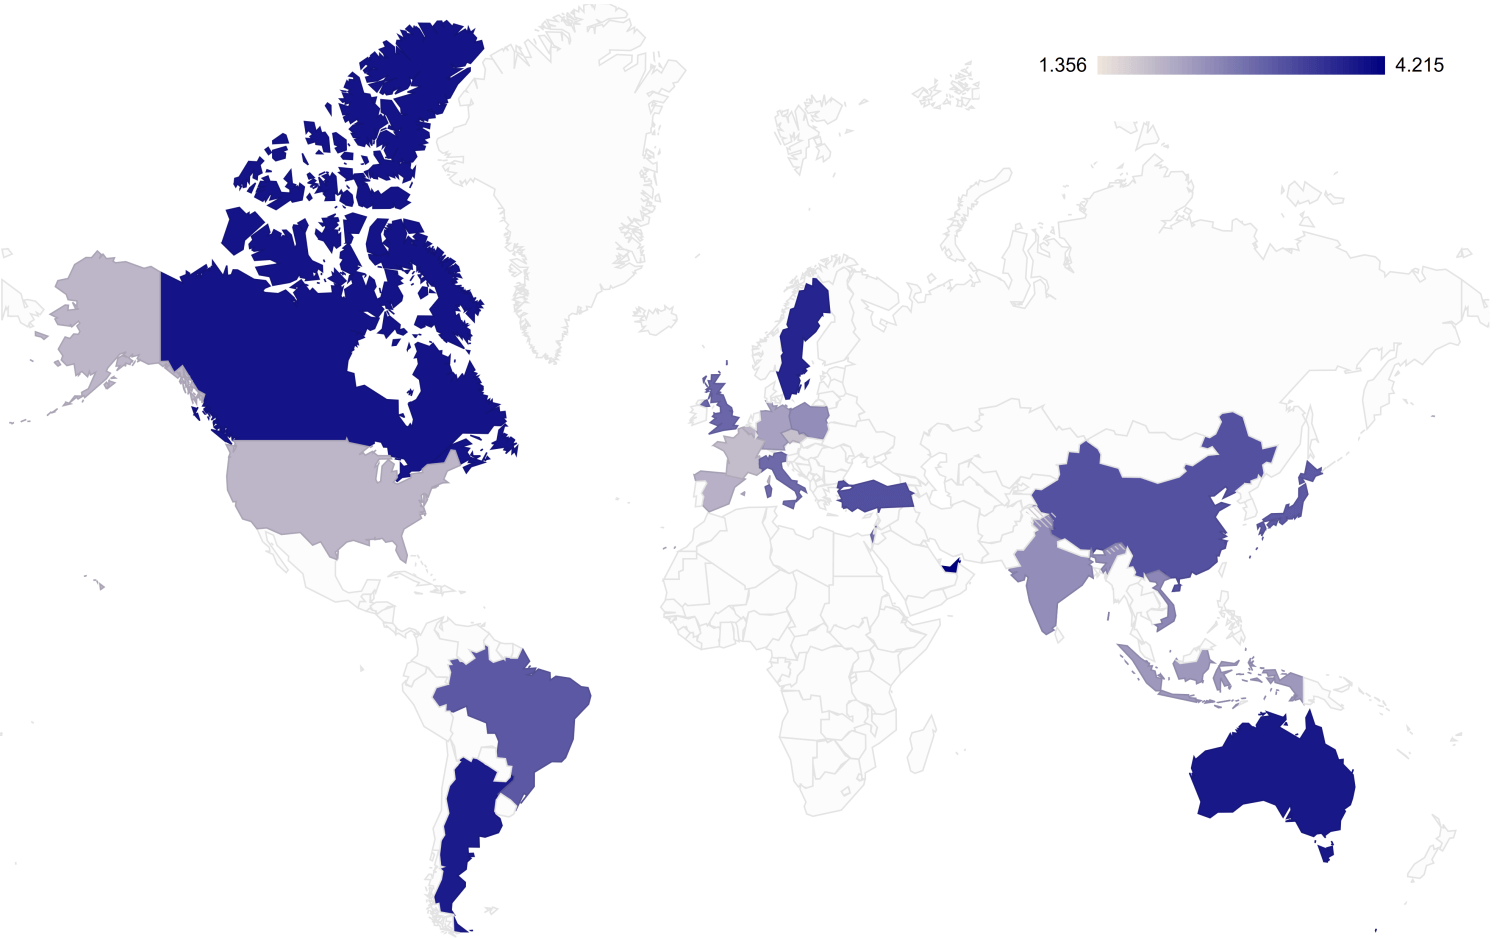
\includegraphics[width=\linewidth]{map.png}
    \caption{Mapa dob načítání} \label{img:Mapa dob načítání}
  \end{figure}

  Z obrázku~\ref{img:Mapa dob načítání} je patrné, že doba načtení webové stránky je do značné míry závislá na vzdálenosti od České republiky, ve které je hostována. Tyto hodnoty rovněž v testovaných zemích výrazně nepřevyšují optimální dobu, což je při uvážení ceny webhostingu přijatelné.


  \subsubsection{Multiplatformnost}
  % TODO: how does the website work on different devices and browsers

  \section{Obsah webové stránky}

  \subsection{Cílová skupina}
  Do cílové skupiny patří lidé v podobné situaci, ve které jsem byl já v roce 2017 při začátku mého členství v \gls{frc} týmu Metal Moose~--~jedinci se zájmem o robotiku, které od studia odrazuje nedostatek intuitivních a lehce pochopitelných materiálů pro studium. Předešlé znalosti v oblasti robotiky či elektrotechniky proto čtení článků stránky potřebné nejsou, doporučeny jsou pouze základní znalosti programování a středoškolské matematiky (geometrie, algebra).


  \subsection{Proces tvorby článků} \label{sec:Proces tvorby článků}
  Při tvorbě nového článku je nejprve zvoleno téma, které bude článek rozebírat. Vyšší prioritu mají témata, jejichž pochopení pro mě bylo z dostupných internetových zdrojů náročné. Další faktory ovlivňující tento výběr jsou obtížnost zařazení tématu do již vytvořených tématických okruhů a jeho použitelnost v soutěži \gls{frc}.

  Po vybrání tématu článku jsou shromážděny dostupné materiály různého druhu~--~prezentace, odborné práce, články, aj. Poté jsou seřazeny podle jejich užitečnosti v mém pochopení daného tématu a na stránce následně zmíněny jako dodatečné studijní materiály.

  Hlavní koncepty těchto témat jsou dále implementovány přes online prostředí RobotMesh v jazyce Python na robotovi ze stavebnice VEX EDR, který byl pro tento účel vytvořen.

  % TODO: add the CAD model x the real model

  Po úspěšném testování a odladění kódu jsou implementace a jejích odvození v článku jednoduchým způsobem (pokud možno obohacené názornými ilustracemi a vizualizacemi) vysvětleny. Na konci je zpravidla rozebírána použitelnost daných konceptů v reálné robotice a nastíněny navazující články v rámci daného tématického okruhu.


  \subsubsection{Vizualizace} \label{sec:Vizualizace}
  Vizualizace jsou implementovány v jazyce JavaScript s využitím knihovny p5.js (viz. kapitola~\fullref{sec:p5.js}). Jsou uzpůsobeny pro ovládání myší či dotykem, aby byly funkční jak na osobních počítačích, tak na mobilech.

  Offline verze stránky vizualizace neobsahuje, protože formát \gls{pdf} vkládání kódu kvůli bezpečnosti neumožňuje~\cite{history-of-pdf}.


  \subsubsection{Ilustrace} \label{sec:Ilustrace}
  Ke tvorbě ilustrací je používán program na tvorbu vektorové grafiky Inkscape (viz. kapitola~\fullref{sec:Inkscape}) v kombinaci s \gls{cad} softwarem Fusion 360 (viz. kapitola~\fullref{sec:Fusion 360}).

  Vektorová grafika je pro vytváření ilustrací správná volba proto, že potřebné tvary lze vytvářet a upravovat výrazně rychleji a efektivněji než rastr. Zabírá také méně místa a je ukládána v prostém textu, což má oproti binárnímu formátu řadu výhod.

  Obrázky~\ref{img:Příklad ilustrace 1},~\ref{img:Příklad ilustrace 2} a~\ref{img:Příklad ilustrace 3} jsou příklady ilustrací, kterými jsou články doprovázeny. Pocházejí z článků o odometrii a ilustrují posunutí robota pro výpočet inverzní kinematiky jeho podvozku.

  \begin{figure}[H]
    \minipage{0.3\textwidth}
      \fbox{
\includegraphics[width=\linewidth]{illustration1.png}}
      \caption{Příklad ilustrace 1} \label{img:Příklad ilustrace 1}
    \endminipage\hfill
     \minipage{0.3\textwidth}
      \fbox{
\includegraphics[width=\linewidth]{illustration2.png}}
      \caption{Příklad ilustrace 2} \label{img:Příklad ilustrace 2}
    \endminipage\hfill
     \minipage{0.3\textwidth}
      \fbox{
\includegraphics[width=\linewidth]{illustration3.png}}
      \caption{Příklad ilustrace 3} \label{img:Příklad ilustrace 3}
    \endminipage
  \end{figure}

  % TODO: write about illustrations

  \subsubsection{Matematika} \label{sec:Matematika}
  Jelikož jsou probírané koncepty a algoritmy založeny na matematice, tak stránka podporuje vkládání rovnic a výrazů do článků. Tuto funkcionalitu zajišťuje JavaScriptová knihovna \KaTeX{} (viz. kapitola~\fullref{sec:KaTeX}), díky které lze \LaTeX ové rovnice umísťovat přímo do Markdownových článků.

  Příkladem zápisu matematiky v článku je rovnice~\ref{eq:katex equation}, která je pomocí \KaTeX u převedena na rovnici~\ref{eq:converted equation}.

  \begin{equation} \label{eq:katex equation}
    \verb|Je pravda, že $$\sum_{i=1}^{n} i = \frac{n(n+1)}{2}$$.|
  \end{equation}

  \begin{equation} \label{eq:converted equation}
    \text{Je pravda, že }\sum_{i=1}^{n} i = \frac{n(n+1)}{2}\text{.}
  \end{equation}


  \subsection{Struktura}
  Stránka je pro ulehčení převodu do \gls{pdf} a plynulosti navigace strukturována do značné míry jako kniha.

  Návštěvníka po zobrazení stránky přivítá \emph{úvodní stránka} (obr.~\ref{img:Úvodní stránka}), která představí projekt a jeho cíle, případně obsahuje důležitá sdělení o provozu stránky. Poté následuje \emph{předmluva} (obr.~\ref{img:Předmluva}), kde jsou kromě diskuzi o předpokladech pro čtení zodpovězeny otázky, které by čtenáři při čtení článků stránky mohli mít.

  \begin{figure}[H]
    \minipage{0.47\textwidth}
      \fbox{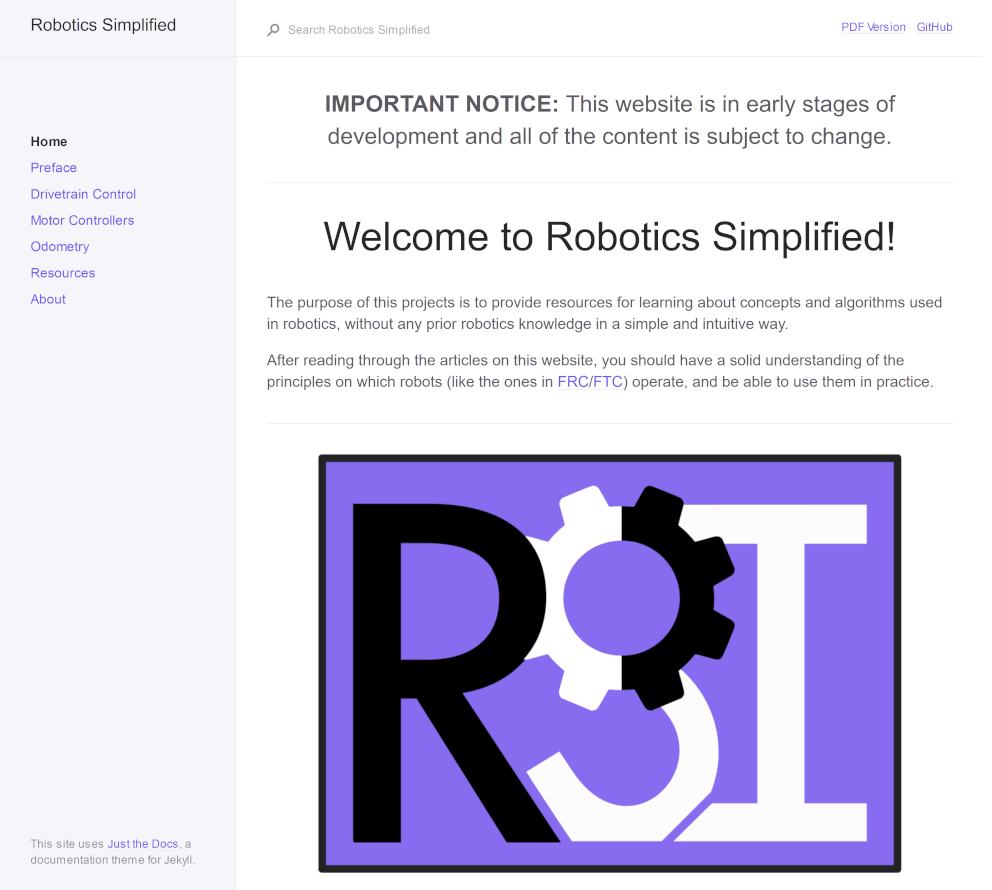
\includegraphics[width=\linewidth]{1.png}}
      \caption{Úvodní stránka} \label{img:Úvodní stránka}
    \endminipage\hfill
     \minipage{0.47\textwidth}
      \fbox{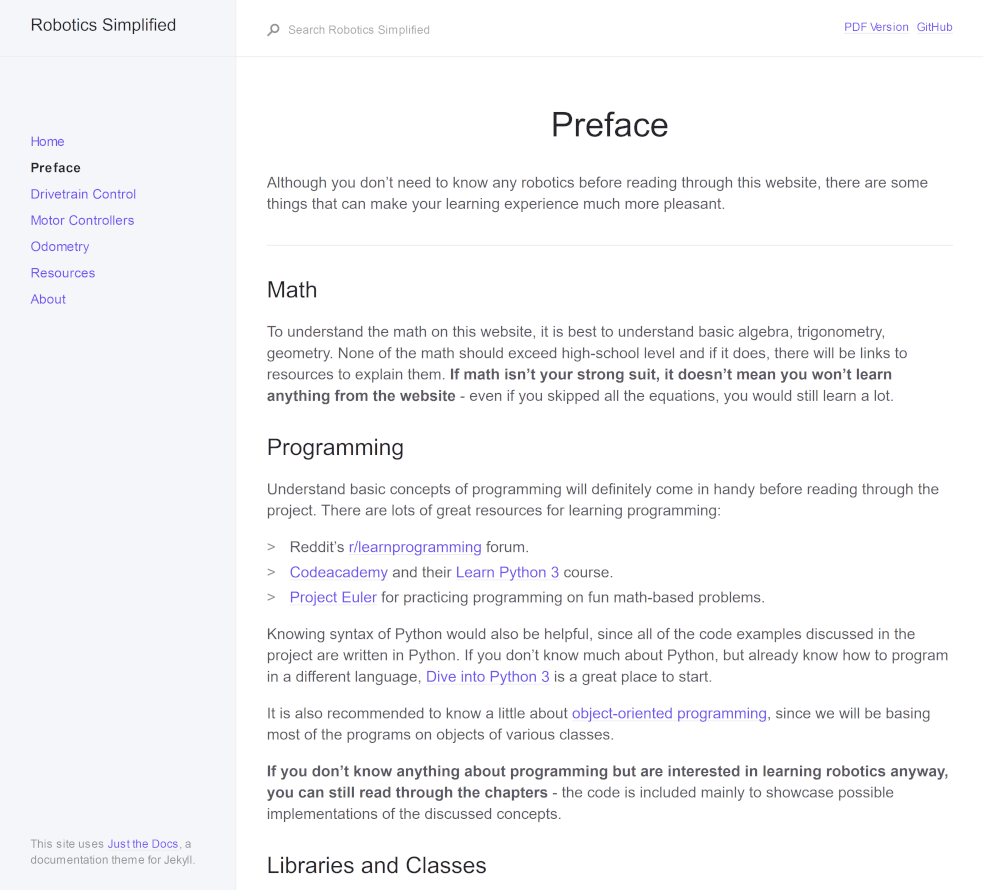
\includegraphics[width=\linewidth]{2.png}}
      \caption{Předmluva} \label{img:Předmluva}
    \endminipage
  \end{figure}

  Hlavní náplní projektu jsou \emph{tématické okruhy} (obr.~\ref{img:Příklad článku 1},~\ref{img:Příklad článku 2},~\ref{img:Příklad článku 3}), které se skládají z článků probírajících koncepty s podobnou tematikou, v pořadí, ve kterém by pro návaznost měly být čteny.

  \begin{figure}[H]
    \minipage{0.3\textwidth}
      \fbox{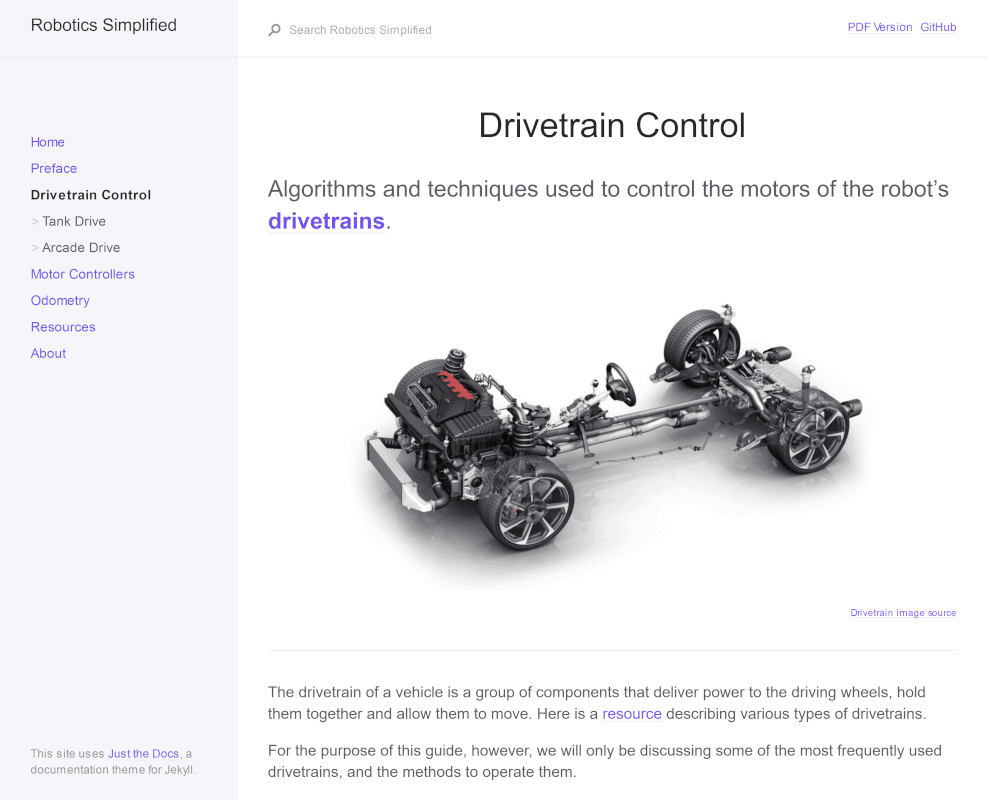
\includegraphics[width=\linewidth]{3-1.png}}
      \caption{Příklad článku 1} \label{img:Příklad článku 1}
    \endminipage\hfill
     \minipage{0.3\textwidth}
      \fbox{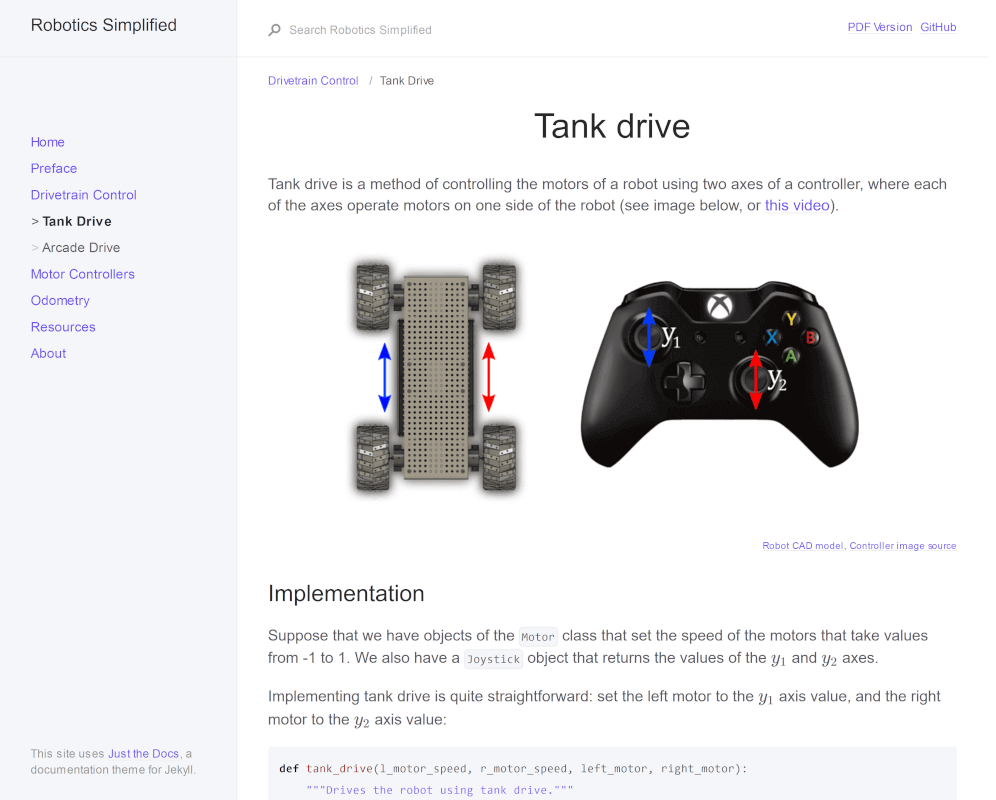
\includegraphics[width=\linewidth]{3-2.png}}
      \caption{Příklad článku 2} \label{img:Příklad článku 2}
    \endminipage\hfill
     \minipage{0.3\textwidth}
      \fbox{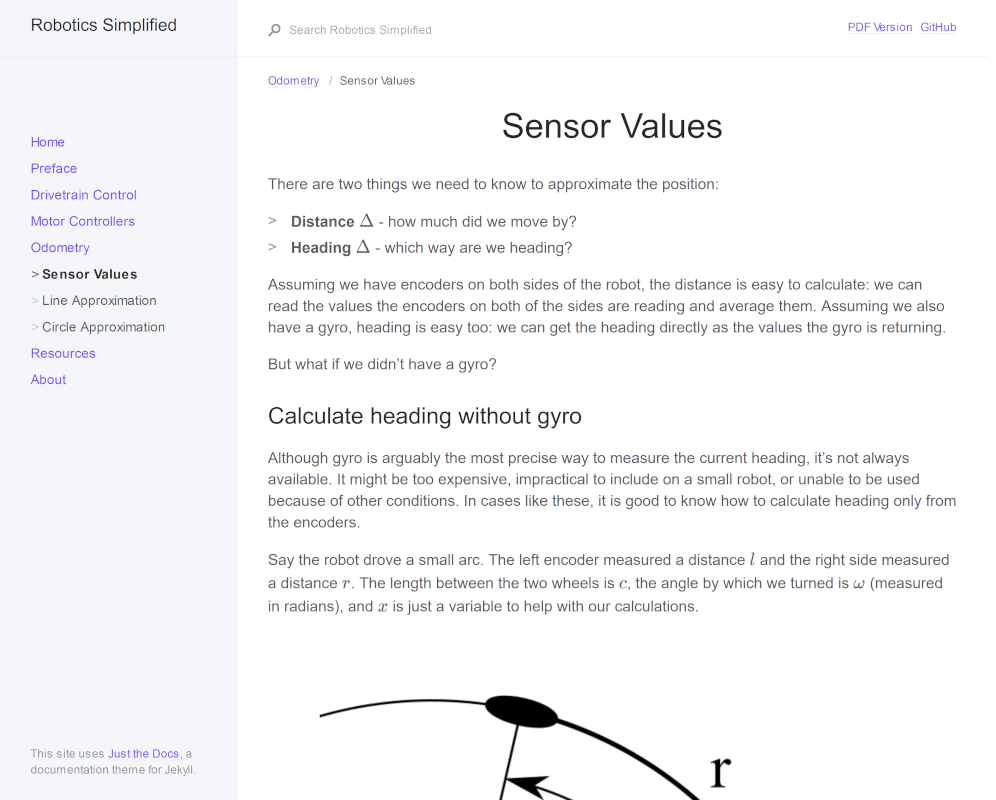
\includegraphics[width=\linewidth]{3-3.png}}
      \caption{Příklad článku 3} \label{img:Příklad článku 3}
    \endminipage
  \end{figure}

  Na závěr je přiložen článek s \emph{odkazy na materiály} (obr.~\ref{img:Odkazy na materiály}) použité při tvorbě projektu a sekce \emph{O nás} (obr.~\ref{img:O nás}), která popisuje důvod za vznikem projektu, návod na případnou spolupráci na projektu a poděkování.

  \begin{figure}[H]
    \minipage{0.47\textwidth}
      \fbox{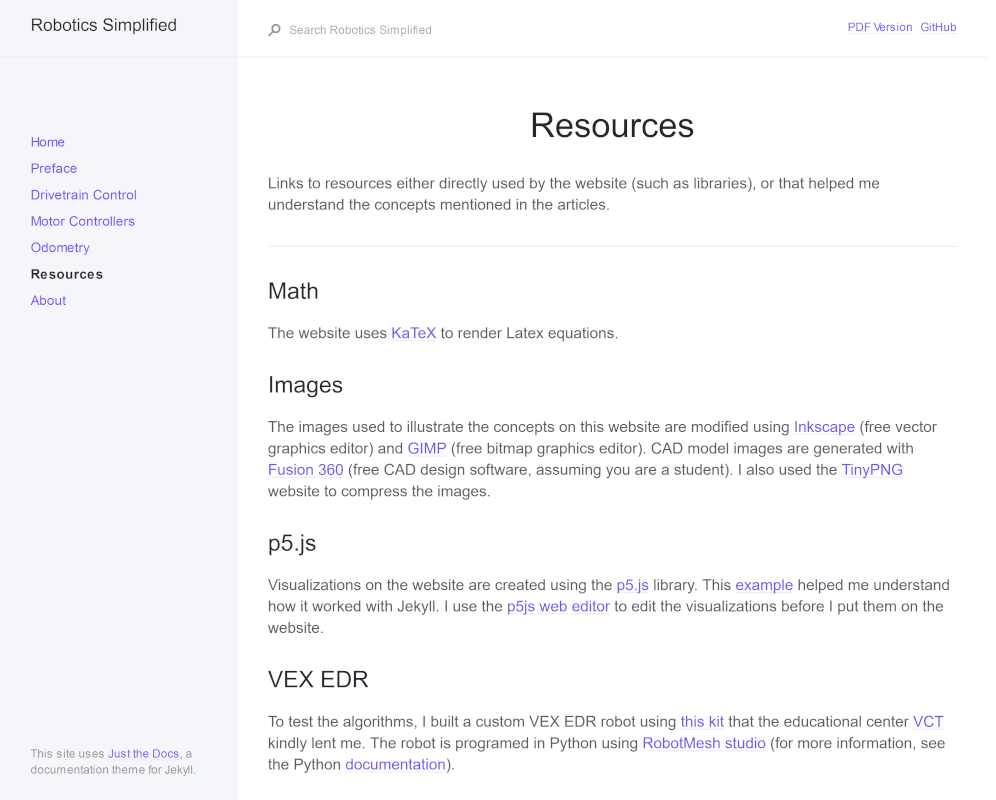
\includegraphics[width=\linewidth]{4.png}}
      \caption{Odkazy na materiály} \label{img:Odkazy na materiály}
    \endminipage\hfill
     \minipage{0.47\textwidth}
      \fbox{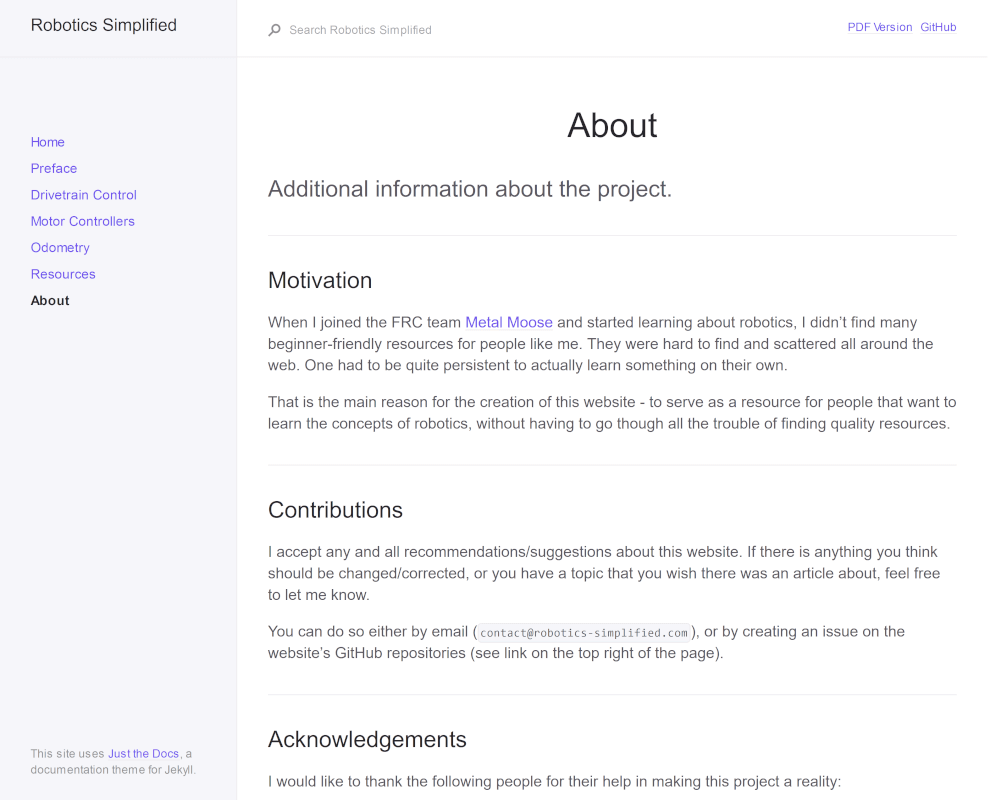
\includegraphics[width=\linewidth]{5.png}}
      \caption{O nás} \label{img:O nás}
    \endminipage
  \end{figure}


  \subsection{Uplatnění}
  Kromě snahy o zpřístupnění robotiky pro nováčky stránka dále poskytuje zdroj strukturovaných vzdělávacích materiálů pro lektory kurzů robotiky a programování. Sám jich několik na Vzdělávacím centru Turnov pomocí této stránky vyučuji a mé zkušenosti byly zatím pouze kladné.

  Díky otevřenosti zdrojového kódu stránka také slouží jako šablona pro Jekyllem poháněné projekty, které by rády docílily obdobné funkcionality (rovnice, automatizace pomocí skriptů, zvýrazňování syntaxe kódu, aj.) bez dlouhavého psaní a ladění kódu.


  \section{Automatizace provozu webové stránky} \label{sec:Automatizace provozu webové stránky}
  Ke tvorbě kvalitního vzdělávacího materiálu je potřeba plynulý a do nejvyšší možné míry automatizovaný provoz stránky~--~k přidání nového článků by mělo stačit v příslušné složce projektu vytvořit nový soubor a zbytek procesu by měl proběhnout bez zásahu autora.

  Stránka je v tomto duchu automatizována skripty psanými v jazyce Python (viz. kapitola~\fullref{sec:Python}), aby se autor mohl plně soustředit na práci.


  \subsection{Nahrání obsahu přes \acrshort{ftp}}
  \gls{ftp} je protokol zprostředkovávající přenos souborů mezi počítači po síti. Od prvního návrhu pro využití na \gls{mit} v roce 1971 až po oficiální specifikaci publikovanou roku 1985 prošel mnoha revizemi a je stále vyvíjen~\cite{ftp-specification}. Jedná se o populární volbu protokolu pro hostingy webových stránek a hosting tohoto projektu není výjimkou.

  Script \texttt{upload.py} se po zadání hesla připojí přes protokol \gls{ftp} na server, rekurzivně smaže soubory a adresáře aktuální verze stránky a nahraje verzi novou. Pro dodatečné zabezpečení je \gls{ip} serveru šifrována symetrickou šifrou \gls{aes}.


  \subsection{Generování souboru sitemap.xml}
  Soubor protokolu sitemap obsahuje informace o pořadí procházení, časech změny a relativní prioritě částí stránky. Slouží vyhledávacím portálům, které tyto soubory využívají pro inteligentnější indexování stránky ve svém systému.

  Script \texttt{sitemap.py} podle pořadí článků generuje záznamy do souboru \texttt{sitemap.xml}. Informace o umístění a poslední úpravě jsou získávány z atributů souborů (článků) a priorita je přidělena podle jejich pozice na stránce~--~úvodní stránka má prioritu $1.0$, hlavní články mají prioritu $0.8$ a vedlejší články prioritu $0.6$.


  \subsection{Převod webové stránky do \acrshort{pdf}} \label{sec:Převod webové stránky do PDF}
  Pro offline dostupnost existuje mnoho různých typů souborů, na které by stránka šla převést. Často používané formáty jako \texttt{doc} a \texttt{docx} jsou však pro použití v projektu nevhodné, protože se mohou na různých zařízeních zobrazit rozdílně. Je tedy vhodnější použít formáty jako PostScript či \gls{pdf}, jejichž vizáž na prostředí závislá není~\cite{history-of-pdf}.

  Přímočará varianta by byla převést články do \gls{pdf} libovolným programem pro převod textových formátů (jako Pandoc). Tímto přístupem by však bylo obtížné generovat obsah a úvodní stránku, a prakticky nemožné ovlivnit výsledné formátování.

  Pro potřeby projektu byl tedy zvolen převod článků do formátu \LaTeX{} (viz. kapitola~\fullref{sec:TeX}) a až poté do formátu \gls{pdf}, což elegantně řeší všechny nevýhody první varianty.

  Script \texttt{tex.py} získá pořadí článků, spojí je za sebe do jednoho dokumentu a poté na ně aplikuje řadu regulárních výrazů, které provedou převod z formátu Markdown do formátu \LaTeX.


  \subsection{Komprimace obrázků}
  O komprimaci obrázků pro zmenšení velikosti stránky se stará skript \texttt{compress.py}, který pomocí služby TinyPNG a jejího Python \gls{api} zkomprimuje všechny obrázky vygenerované stránky. Samotný \gls{api} klíč je pro zamezení zneužití šifrován symetrickou šifrou \gls{aes}.

  Úprava fotek funguje na principu \emph{kvantování barev}~--~podobné barvy jsou spojeny do jedné, čímž lze z tradičních 24-bitových palet \gls{png} obrázků udělat palety 8-bitové a zmenšit tím obrázek bez výrazného zhoršení kvality.

  Ke 24. únoru 2019 tento skript zkomprimuje obrázky webové stránky na $72.3$ \% jejich původní velikosti a zmenší tím její velikost o \emph{262 KB}.


  \subsection{Minimalizace zdrojového kódu}
  Zkompaktnění zdrojového kódu je další možná optimalizace, kterou lze načítání stránky urychlit. Prohlížečům na vzhledu kódu nezáleží a běžné uživatele nezajímá, proto jej lze na úkor čitelnosti zmenšit.

  Tuto funkci zastává skript \texttt{minify.py}, který soubory typu \gls{css} a \gls{html} zmenší odstraněním komentářů, nepotřebných tagů a uvozovek, přebytečných mezer a dalších částí kódu, které po jejich odstranění funkcionalitu kódu nezmění.

  Ke 24. únoru 2019 tento skript zkompaktní \gls{css} a \gls{html} webové stránky na $72.89$ \% a $68.12$ \% jejich původní velikosti a zmenší tím její velikost o \emph{129 KB}.


  \subsection{Automatizace procesu}
  Po přidání či úpravě článku je potřeba verzi stránky na hostingu aktualizovat. Tento proces řídí skript \texttt{deploy.py}, který stránku nejprve pomocí Jekyllu vygeneruje, poté ve správném pořadí spustí všechny skripty pro generování dodatečného obsahu a optimalizace a nakonec i skript pro nahrání stránky na webhosting.


  \section{Analytika a propagace webové stránky}
  % TODO: how is traffic analysis and marketting done

  \subsection{Analýza návštěvnosti}

  \subsubsection{Google Analytics}
  Google Analytics je služba společnosti Google. Slouží k analýze návštěvnosti webových stránek. Pro použití stačí na danou stránku přidat JavaScriptovou knihovnu % TODO: finish writing this

  % TODO: add location pie chart
  % TODO: add device pie chart
  % TODO: add age pie chart
  % TODO: add gender pie chart


  \subsubsection{Google Search Console}
  Kromě služby Google Analytics rozebírané v předešlé kapitole k slouží získávání statistik o webové stránce služba Google Search Engine, která zobrazuje statistiky o indexování webové stránky v rámci vyhledávání Google~--~její průměrné pozice při relevantních vyhledáváních, počet zobrazení, indexované podstránky, aj.


  \subsection{Marketting}

  \subsubsection{Sociální média}
  K získání zpětné vazby o technicky zaměřeném projektu je vhodné použít webové stránky s obdobnou tématikou. Projekt byl z tohoto důvodů zveřejněn na následujících internetových fórech:

  {\parskip=0pt
  \begin{itemize}[topsep=\itemsep]
    \item \emph{ChiefDelphi}~--~internetové fórum zaměřené na soutěž \gls{frc}, převážně pro členy \gls{frc} týmů.
    \item \emph{Reddit}~--~jedno z nejpopulárnějších internetových fór dneška. Zajímavostí jsou subreddity~--~samospravované celky, na kterých jsou zveřejňovány články se společnou tématikou.
    \begin{itemize}[topsep=0pt]
      \item \emph{Subreddit \gls{frc}}~--~zaměření na soutěž \gls{frc}, od vtipných obrázků a videí po odborné články. Časté jsou též novinky a události ze světa soutěže.
      \item \emph{Subreddit Robotics}~--~většina příspěvků jsou vzdělávacího charakteru. Časté druhy příspěvků jsou videa a články o domácích projektech uživatelů tohoto fóra.
    \end{itemize}
    \item \emph{Hacker News}~--~internetové fórum, které je ve svém fungování blízké Redditu. Není však dále strukturováno na subreddity a obsah je vážnějšího charakteru~--~světové novinky, nové výzkumy a odborné práce, měsíční přehledy dostupných pracovních pozic \gls{it} firem, apod.
  \end{itemize}}


  \subsubsection{\acrshort{frc} a \acrshort{fll} týmy}

  \newpage

  \section{Závěr}
  Náplní práce na projektu je v dohledné budoucnosti tvorba nových článků a jejich lokalizace do českého jazyka. S tím je též úzce spjata revize již napsaných článků~--~přidávání dodatečných ilustrací a vizualizací, zpřehlednění textu, revize kódu, aj.

  Stránka rovněž prozatím nepoužívá protokol \gls{https}, který narozdíl od \gls{http} šifruje komunikaci mezi klientem a serverem a zamezuje tím řadě možných útoků, před kterými \gls{http} uživatele nechrání. Jelikož však WEDOS podporuje mezinárodně uznávanou certifikační autoritu Let's Encrypt, tak by tato změna neměla být složitá.

  Další oblastí zlepšení je převod webové stránky do offline verze~--~přidání dodatečných formátů jako \gls{epub} a \gls{mobi} pro zlepšení podpory elektronických čteček knih, zajištění větší spolehlivosti převodu a přidání dalších funkcí (přeškrtnutí textu, podtržení textu, reference, citace...).

  Jedna z dalších možných úprav by byla nahrazení knihovny p5.js za kód využívající pouze JavaScript canvas kvůli zmenšení velikostí článků obsahující vizualizace, jelikož velikost samotné knihovny je \emph{451 KB}.


  \newpage

  % create the bibliography
  \printbibliography[heading=bibnumbered, title=Použitá literatura]

  \newpage

  % create lof and lot
  \section{Seznam obrázků a tabulek}
  {%
  \let\oldnumberline\numberline%
  \renewcommand{\numberline}{\figurename~\oldnumberline}%
  \listoffigures%
  }
  \vspace{\baselineskip}
  {%
  \let\oldnumberline\numberline%
  \renewcommand{\numberline}{\tablename~\oldnumberline}%
  \listoftables%
  }

  \newpage

  \section{Příloha 1: Data testování doby načtení} \label{sec:Příloha 1: Data testování doby načtení}
  Následující tabulka obsahuje místa, ze kterých byla testována doba načtení stránky \url{http://robotics-simplified.com/} a častečné odkazy na testovací data. K vytvoření úplného odkazu stačí před označení daného města přidat \texttt{www.webpagetest.org/result/}.

\begin{table}[H]
  \centering
  \begin{tabular}{*5l}  \toprule
    \emph{Město}            & \emph{Označení}                      \\ \midrule
    Buenos Aires, Argentina & \href{https://www.webpagetest.org/result/190213_PC_5d05753a2ce2126089db6b8726171c13}{\texttt{190213\_PC\_5d05753a2ce2126089db6b8726171c13}} \\
    Toronto, Canada         & \href{https://www.webpagetest.org/result/190213_44_a861d3caa2bdbb547775b76e0ca7e357}{\texttt{190213\_44\_a861d3caa2bdbb547775b76e0ca7e357}} \\
    La Rioja, Spain         & \href{https://www.webpagetest.org/result/190213_ZA_96b8ca66a5af8d0bbee48a48d1ebf901}{\texttt{190213\_ZA\_96b8ca66a5af8d0bbee48a48d1ebf901}} \\
    Prague, Czech Republic  & \href{https://www.webpagetest.org/result/190213_SD_119a43e321c4360178004f09bb4d27a0}{\texttt{190213\_SD\_119a43e321c4360178004f09bb4d27a0}} \\
    London, UK              & \href{https://www.webpagetest.org/result/190213_SS_1226a99822746d3cf16fb81bd19c9ac8}{\texttt{190213\_SS\_1226a99822746d3cf16fb81bd19c9ac8}} \\
    Strasburg, France       & \href{https://www.webpagetest.org/result/190213_35_5db33eb4e90d8b096d8853fa453d54d3}{\texttt{190213\_35\_5db33eb4e90d8b096d8853fa453d54d3}} \\
    Brussels, BE            & \href{https://www.webpagetest.org/result/190213_PK_8973798f51f040a199501b3332071bc2}{\texttt{190213\_PK\_8973798f51f040a199501b3332071bc2}} \\
    Berlin, Germany         & \href{https://www.webpagetest.org/result/190213_S3_321db7231844fc993d91fba974e569bb}{\texttt{190213\_S3\_321db7231844fc993d91fba974e569bb}} \\
    Milan, Italy            & \href{https://www.webpagetest.org/result/190213_QE_7d2d0c62fe56d0a992f83872fea9589a}{\texttt{190213\_QE\_7d2d0c62fe56d0a992f83872fea9589a}} \\
    Warsaw, Poland          & \href{https://www.webpagetest.org/result/190213_AV_e12420619d2b67b02b36fd8f85012634}{\texttt{190213\_AV\_e12420619d2b67b02b36fd8f85012634}} \\
    Stockholm, Sweden       & \href{https://www.webpagetest.org/result/190213_PC_8bf596590b3cb93164fb6b20e2ae9b7a}{\texttt{190213\_PC\_8bf596590b3cb93164fb6b20e2ae9b7a}} \\
    Istanbul, Turkey        & \href{https://www.webpagetest.org/result/190213_FZ_3eb94a70dfdd8c92bcfcfaf74a412501}{\texttt{190213\_FZ\_3eb94a70dfdd8c92bcfcfaf74a412501}} \\
    Israel                  & \href{https://www.webpagetest.org/result/190213_XT_735a3f35ee6a8056ad47aac3d5a95917}{\texttt{190213\_XT\_735a3f35ee6a8056ad47aac3d5a95917}} \\
    Dubai, UAE              & \href{https://www.webpagetest.org/result/190213_66_d158a4ae09a1ef5d63b68693b5230066}{\texttt{190213\_66\_d158a4ae09a1ef5d63b68693b5230066}} \\
    Seoul, Korea            & \href{https://www.webpagetest.org/result/190213_TX_d56f64b9948b96bdfdd1323fd16b0867}{\texttt{190213\_TX\_d56f64b9948b96bdfdd1323fd16b0867}} \\
    Mumbai, India           & \href{https://www.webpagetest.org/result/190213_ED_2a0542955442372c423c9306a7492c02}{\texttt{190213\_ED\_2a0542955442372c423c9306a7492c02}} \\
    Amsterdam, NL           & \href{https://www.webpagetest.org/result/190213_37_88f29978d6231e700fe963b8d943a79b}{\texttt{190213\_37\_88f29978d6231e700fe963b8d943a79b}} \\
    Sydney, Australia       & \href{https://www.webpagetest.org/result/190213_8N_c4802d60f2820dd2b7f8e3e5d6a384c1}{\texttt{190213\_8N\_c4802d60f2820dd2b7f8e3e5d6a384c1}} \\
    Clifton, NJ             & \href{https://www.webpagetest.org/result/190213_3S_570bc4b76dd084486a1ae6ba1829f2cc}{\texttt{190213\_3S\_570bc4b76dd084486a1ae6ba1829f2cc}} \\
    Jakarta, Indonesia      & \href{https://www.webpagetest.org/result/190213_12_db0913a1b2708f54db46d5d40b7f61e5}{\texttt{190213\_12\_db0913a1b2708f54db46d5d40b7f61e5}} \\
    Tokyo, Japan            & \href{https://www.webpagetest.org/result/190213_8Q_083b45677c2c51f4fe7bd25b554dff38}{\texttt{190213\_8Q\_083b45677c2c51f4fe7bd25b554dff38}} \\
    Sao Paulo, Brazil       & \href{https://www.webpagetest.org/result/190213_AD_d2d6ea6b39f36853cf476a5f1d1f3092}{\texttt{190213\_AD\_d2d6ea6b39f36853cf476a5f1d1f3092}} \\
    Vietnam                 & \href{https://www.webpagetest.org/result/190213_RQ_18f2a02931599884f8922a3ce09f56bc}{\texttt{190213\_RQ\_18f2a02931599884f8922a3ce09f56bc}} \\
    Hong Kong, China        & \href{https://www.webpagetest.org/result/190213_NK_dfd8ddf4b9766b3386799de124a67ad8}{\texttt{190213\_NK\_dfd8ddf4b9766b3386799de124a67ad8}} \\ \bottomrule \hline
  \end{tabular}
  \label{tab:Data testování doby načtení}
  \caption{Data testování doby načtení}
\end{table}

\end{document}
